\section{Singleton-Muster}
\subsection{Definition}
Das Singleton-Muster sicher, dass es nur eine Instanz einer Klasse gibt, und bietet einen globalen 
Zugriffspunkt fuer diese Instanz. 

\subsection{Erklaerung}
\begin{itemize}
\item Wir nehmen eine Klasse und lassen sie eine einzige Instanz von sich selbst verwalten. Wir 
  verhindern auch, dass irgendeine andere Klasse eigenstaendig eine neue Instanz erstellt. Um eine 
  Instanz zu erhalten, muss man ueber die Klasse selbst gehen. 
\item Wir bieten ausserdem einen globalen Zugriffspunkt fuer die Instanz: Jedes Mal wenn Sie eine 
  Instanz benoetigen, fragen Sie einfach be der Klasse nach, und diese reicht Ihnen, die eine 
  Instanz. Wie Sie gesehen haben, koennen wir das so implementieren, dass das Singleton verzoegert 
  erstellt werden kann, was bei ressourcenintensiven Objekten besonders wichtig ist. 
\end{itemize}

\FloatBarrier

\begin{figure}[h]
	\centering
	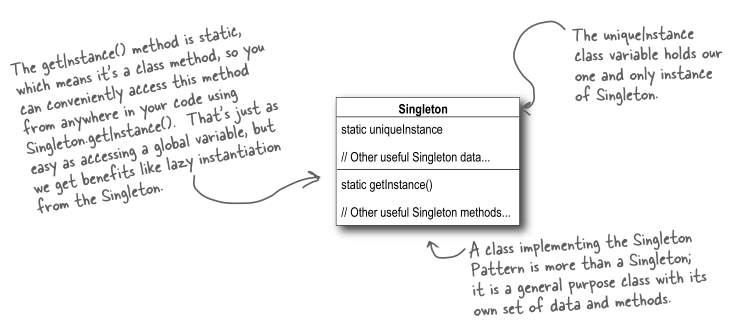
\includegraphics[width=.8\linewidth]{singleton/img/singletonUML}
	\caption{UML-Darstellung des \emph{einfachen} Singleton-Musters}
	\label{fig:singletonUML}
\end{figure}